\section{Bayesian filter}

As the robot navigates from an initial position to a target destination along a specific path, it's essential to integrate both its motion and sensor models effectively. 
Bayesian filtering provides a method to achieve this integration seamlessly.

The motion model encompasses the robot's pose $\Gamma$ and the actions it takes $u$. 
Meanwhile, the sensor model incorporates the robot's pose $\Gamma$, observations $z$, and the map of the environment $L$. 
\begin{figure}[H]
    \centering
    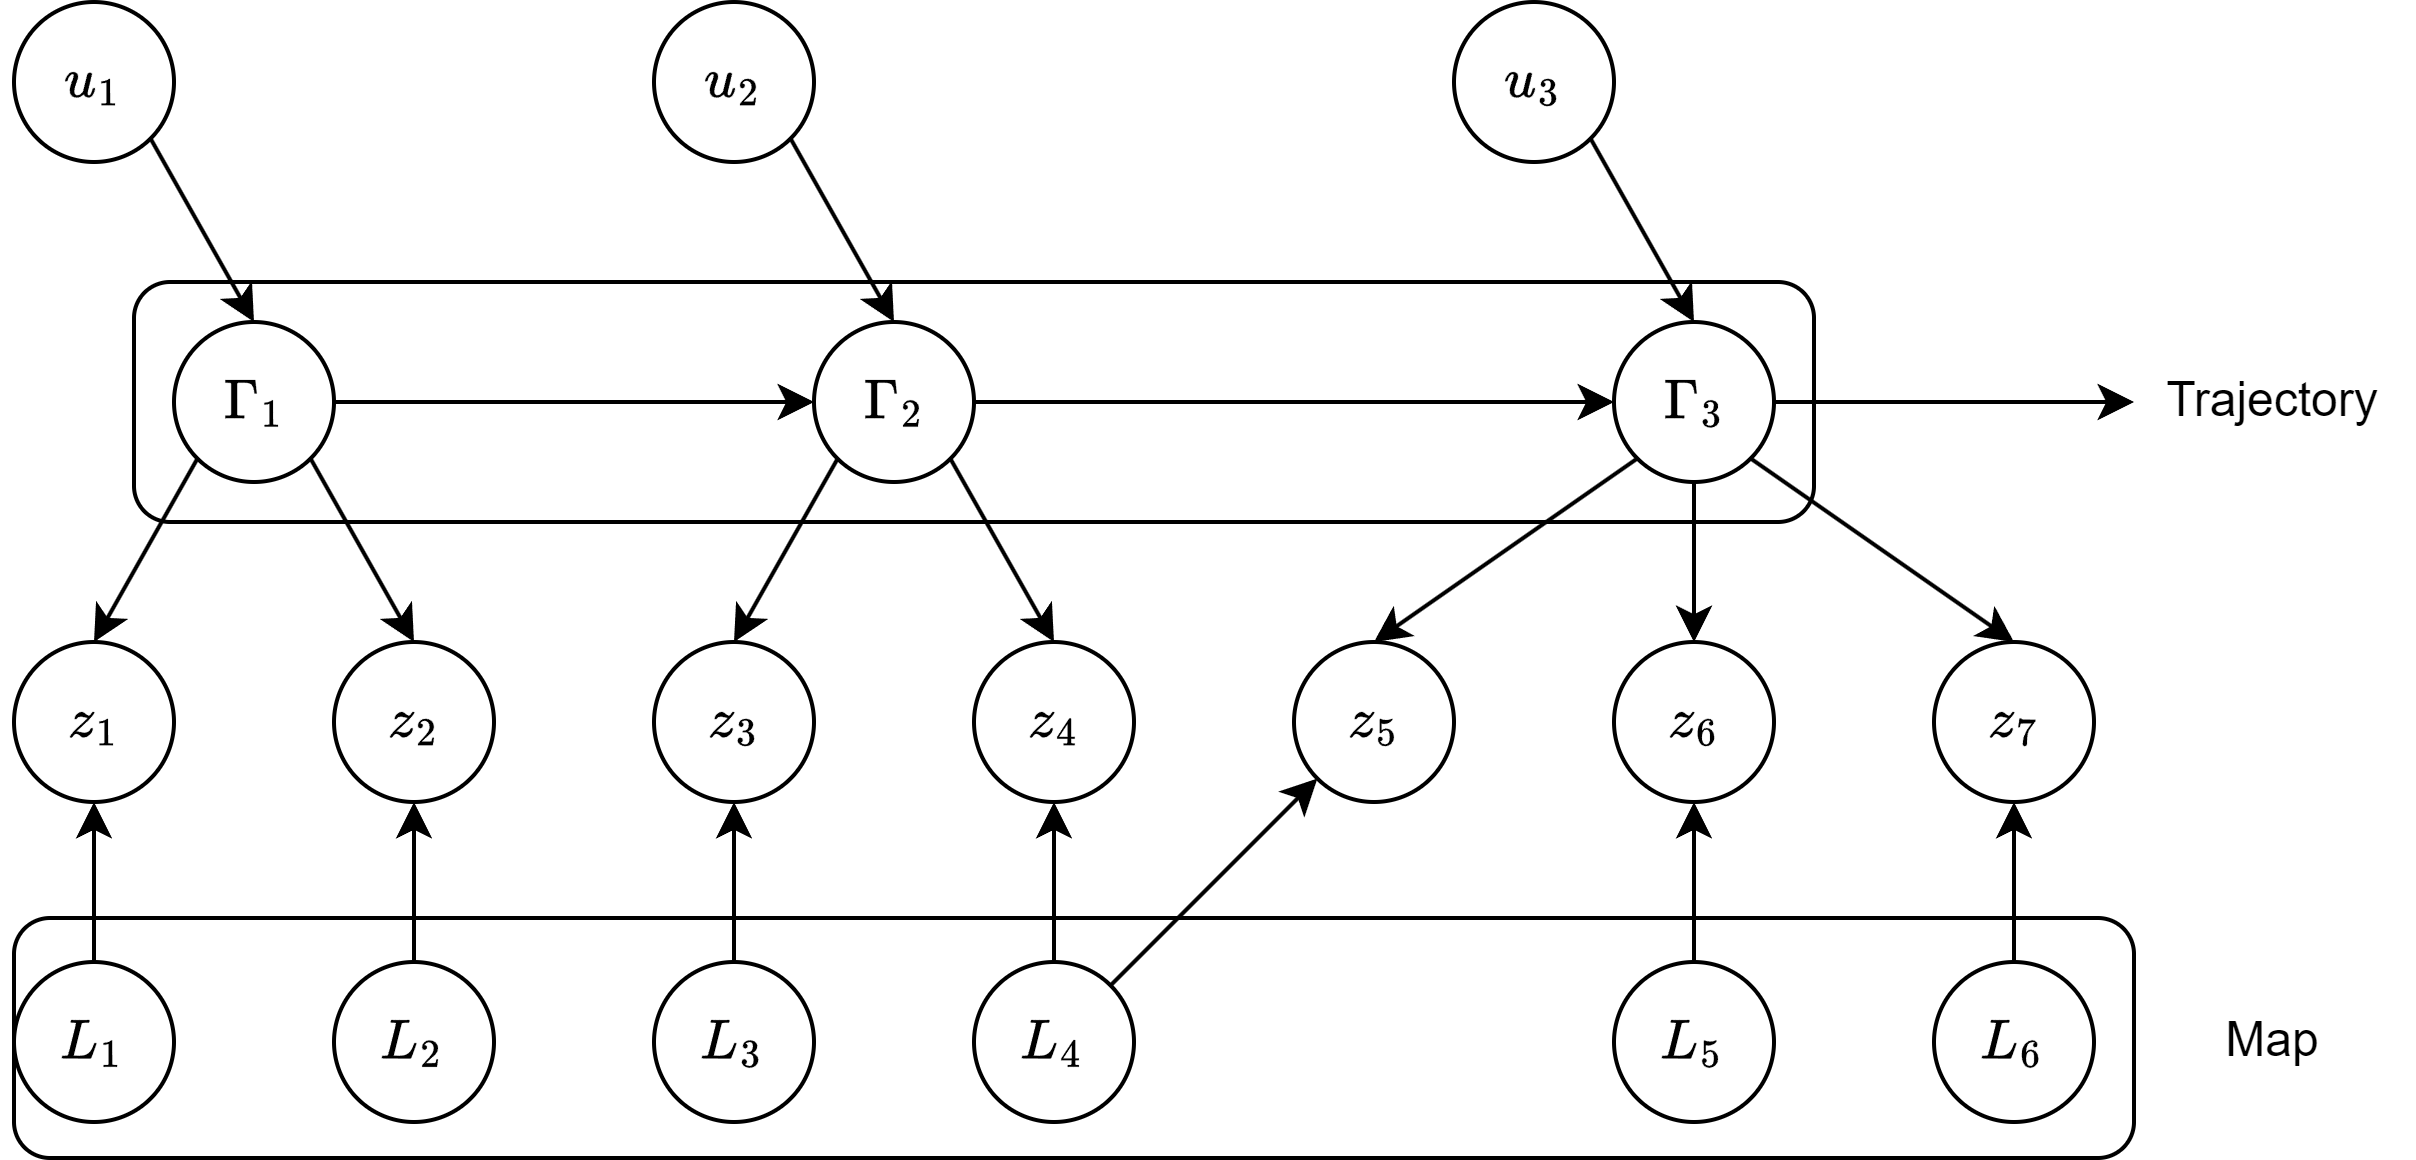
\includegraphics[width=0.75\linewidth]{images/slam.png}
    \caption{Localization framework}
\end{figure}
The filtering process aims to estimate the posterior probability distribution of the robot's state $x(t)$ given the stream of information about movement and sensors 
$d_t=\left\{u_1,z_1,\dots,u_t,z_t\right\}$ and the map of the environment $m$.
We have the motion model which provides the probability distribution $\Pr(\Gamma_t|\Gamma_{t:1},l_1,\dots,l_n)$ representing the robot's pose at time $t$ given its past poses and the map.
Our goal is to compute the belief $\text{Bel}(x_t)=P(x_t|u_1,z_1,\dots,u_t,z_t,m)$ representing the probability distribution of the robot's state $x_t$ given all the available information.
To compute $\text{Bel}(x_t)$, we typically use Bayes' rule, incorporating both the motion and sensor models. The motion model predicts the next state given the current state and action, while the sensor model updates this prediction based on the observations. This recursive process allows us to continuously refine our estimate of the robot's state as new information becomes available.

\paragraph*{Assumptions}
We make the following assumptions, all of which are known:
\begin{itemize}
    \item The prior probability of the system state $\Pr(x_0)$. 
    \item The motion model $\Pr(x^\prime|x, u)$, which describes the probability of transitioning from state $x$ to state $x^\prime$ given action $u$.
    \item The sensor model $\Pr(z|x, m)$, which describes the probability of obtaining observation $z$ given the system state $x$ and the map $m$.
\end{itemize}

\paragraph*{Markov assumption}
Additionally, we require the Markov assumption:
\begin{property}
    A stochastic process possesses the Markov property if the conditional probability distribution of future states, conditioned on both past and present values, depends solely on the present state.
\end{property}
In other words, given the present state, the future states are independent of the past.

Furthermore, we assume:
\begin{itemize}
    \item Perfect model: the models accurately represent the system and environment.
    \item No approximation errors: the computations are exact.
    \item Static and stationary world: the environment does not change over time.
    \item Independent noise: the noise in sensor readings and system dynamics is independent and identically distributed.
\end{itemize}


\subsection{Bayes filter}
With the given assumptions, we can derive the belief on the robot's position using Bayes' theorem:
\begin{align*}
    \text{Bel}(x_t) &=\Pr(x_t,z_1,\dots,u_t,z_t,m) \\
                    &=\eta\Pr(z_t|x_t,u_1,z_1,\dots,u_t,m)\Pr(x_t|u_1,z_1,\dots,u_t,m) 
\end{align*}
Using the Markov property and Bayes' rule, we simplify further:
\[\text{Bel}(x_t)=\eta\Pr(z_t|x_t,m)\Pr(x_t|u_1,z_1,\dots,u_t,m)\]
Expanding the second term using the recursive Bayes filter equation:
\[\text{Bel}(x_t)=\eta\Pr(z_t|x_t,m)\int\Pr(x_t|u_1,z_1,\dots,u_t,x_{t-1},m)\Pr(x_{t-1}|u_1,z_1,\dots,u_{t-1},m)\,dx_{t-1}\]
Applying the Markov property again and simplifying:
\[\text{Bel}(x_t)=\eta\Pr(z_t|x_t,m)\int\Pr(x_t|u_t,x_{t-1})\Pr(x_{t-1}|u_1,z_1,\dots,u_{t-1},m)\,dx_{t-1}\]
Now, recognizing that the belief at $x_{t-1}$ is the same as $\text{Bel}(x_{t-1})$, we can rewrite the integral:
\[\text{Bel}(x_t)=\eta\Pr(z_t|x_t,m)\int\Pr(x_t|u_t,x_{t-1})\text{Bel}(x_{t-1})\,dx_{t-1}\]
In this expression, $z$ represents an observation, $u$ represents an action, $x$ represents a state, and $m$ represents a map.
This recursive formulation allows us to iteratively update our belief about the robot's position based on new sensor readings and actions.

\subsection{Bayes filter algorithm}
The Bayes filter algorithm computes the belief of a certain position $x$ given perceptual data $z$ or action data $u$. 
If the map is given, the belief at $x_t$ is updated using the formula:
\[\text{Bel}(x_t|m)=\eta\Pr(z_t|x_t,m)\int\Pr(x_t|u_t,x_{t-1},m)\text{Bel}(x_{t-1}|m)\,dx_{t-1}\]
Here's the Bayes filter algorithm:
\begin{algorithm}[H]
    \caption{Bayes filter algorithm}
        \begin{algorithmic}[1]
            \If{$d$ is a perceptual data item $z$} 
                \For{all $x$}
                    \State{$\text{Bel}^\prime(x)=\Pr(z|x)\text{Bel}(x)$}
                \EndFor
                \State{normalize $\text{Bel}^\prime(x)$}
            \ElsIf{$d$ is an action data item $u$}
                \For{all $x$}
                    \State{$\text{Bel}^\prime(x)=\int\Pr(x|u,x^\prime)\text{Bel}(x^\prime)\,dx^\prime$}
                \EndFor
            \EndIf
            \State \Return{$\text{Bel}^\prime(x)$}
        \end{algorithmic}
\end{algorithm}
This algorithm updates the belief state based on either a perceptual data item $z$ or an action data item $u$. 
If $d$ is a perceptual data item, it computes the product of the probability of observation given each state and the current belief state, then normalizes the result.
If $d$ is an action data item, it integrates over the motion model to update the belief state.

Based on this representation, various filtering algorithms can be implemented, including discrete filters, Kalman filters, sigma-point filters, and particle filters. 
These algorithms differ in how they represent and update the belief state and handle uncertainties in the system and sensor measurements.

\subsection{Discrete Bayes filter algorithm}
The discrete Bayes filter algorithm provides a method for updating the belief state when the map is discretized into regions. 
Here's the algorithm:
\begin{algorithm}[H]
    \caption{Discrete Bayes filter algorithm}
        \begin{algorithmic}[1]
            \State{$h=0$}
            \If{$d$ is a perceptual data item $z$} 
                \For{all $x$}
                    \State{$\text{Bel}^\prime(x)=\Pr(z|x)\text{Bel}(x)$}
                    \State{$\eta=\eta+\text{Bel}^\prime(x)$}
                \EndFor
                \For{all $x$}
                    \State{$\text{Bel}^\prime(x)=\eta^{-1}\text{Bel}^\prime(x)$}
                \EndFor
                \State{normalize $\text{Bel}^\prime(x)$}
            \ElsIf{$d$ is an action data item $u$}
                \For{all $x$}
                    \State{$\text{Bel}^\prime(x)=\sum_{x^\prime}\Pr(x|u,x^\prime)\text{Bel}(x^\prime)$}
                \EndFor
            \EndIf
            \State \Return{$\text{Bel}^\prime(x)$}
        \end{algorithmic}
\end{algorithm}
This algorithm updates the belief state based on either a perceptual data item $z$ or an action data item $u$: 
\begin{itemize}
    \item When the data item $d$ is a perceptual input $z$, the algorithm computes the product of the probability of observation given each state and the current belief state. 
        Then, it normalizes the resulting belief to ensure it sums to one.
    \item When $d$ represents an action $u$, the algorithm updates the belief state by summing over all possible previous states $x^\prime$ weighted by the transition probabilities $\Pr(x|u,x^\prime)$.
\end{itemize}
The algorithm facilitates belief update upon sensory input and normalization, iterating over all cells. 
For efficiency, especially when the belief is peaked (e.g., during position tracking), it's advisable to avoid updating irrelevant parts. 
Instead, focus on updating relevant components based on the likelihood of observations given the active components.

For updating the belief upon robot motion, the algorithm assumes a bounded Gaussian model to reduce the computational complexity from $O(n^2)$ to $O(n)$. 
This involves shifting the data in the grid according to the measured motion and then convolving the grid using a Gaussian kernel.